\documentclass[10pt,a4paper]{article}
\usepackage{graphicx}
\usepackage{subfig}
\usepackage{svg}

%%%%%%%%%%%%%%%%%%%%%%%%%%%
% MODIFY:

\newcommand{\authorA}{Jia Long Ji Qiu}
\newcommand{\authorB}{Jiabo Wang}
\newcommand{\authorC}{Yilun Liu}
\newcommand{\groupNumber}{J} % - YOUR GROUP NUMBER
\newcommand{\exerciseNumber}{3} % - THE NUMBER OF THE EXERCISE
\newcommand{\sourceCodeLink}{https://github.com/jialongjq/mlcms}

\newcommand{\workPerAuthor}{
\authorA&Task 1&1/3\\
      &Task 2&1/3\\
      &Task 3&1/3\\
      &Task 4&1/3\\
      \hline
\authorB&Task 1&1/3\\
      &Task 2&1/3\\
      &Task 3&1/3\\
      &Task 4&1/3\\
      \hline
\authorC&Task 1&1/3\\
      &Task 2&1/3\\
      &Task 3&1/3\\
      &Task 4&1/3\\
}

%%%%%%%%%%%%%%%%%%%%%%%%%%%

%%
% imports for the exercise sheets
%

\usepackage[utf8]{inputenc}
\usepackage{amsmath}
\usepackage{amsfonts}
\usepackage{amssymb}

\usepackage[yyyymmdd]{datetime}
\renewcommand{\dateseparator}{--}

\usepackage[left=2cm,right=2cm,top=3cm,bottom=3cm]{geometry}
\usepackage{listings, xcolor}

\definecolor{codegreen}{rgb}{0,0.6,0}
\definecolor{codegray}{rgb}{0.5,0.5,0.5}
\definecolor{codepurple}{rgb}{0.58,0,0.82}
\definecolor{backcolour}{rgb}{0.95,0.95,0.92}

\lstdefinestyle{mystyle}{
    backgroundcolor=\color{backcolour},   
    commentstyle=\color{codegreen},
    keywordstyle=\color{magenta},
    numberstyle=\tiny\color{codegray},
    stringstyle=\color{codepurple},
    basicstyle=\ttfamily\footnotesize,
    breakatwhitespace=false,         
    breaklines=true,                 
    captionpos=b,                    
    keepspaces=true,               
    showspaces=false,                
    showstringspaces=false,
    showtabs=false,                  
    tabsize=2
}

\lstset{style=mystyle}

\usepackage{hyperref}

\usepackage{amsthm}
\newtheorem{lem}{Lemma}
\newtheorem{thm}{Theorem}
\newtheorem{cor}{Corollary}
\newtheorem{rem}{Remark}
\newtheorem{definition}{Definition}
\newtheorem{ter}{Terminology}

\usepackage{graphicx}

\newcommand{\M}{\mathcal{M}}
\newcommand{\N}{\mathcal{N}}
\newcommand{\K}{\mathcal{K}}
\newcommand{\SPDk}{\mathbb{P}^k}
\newcommand{\vol}{\text{vol}}

\newcommand{\Figref}[1]{Figure~\ref{#1}}
\newcommand{\figref}[1]{figure~\ref{#1}}
\newcommand{\Eqnref}[1]{Equation~(\eqref{#1})}
\newcommand{\eqnref}[1]{equation~(\eqref{#1})}

\usepackage{float}
\usepackage{tabularx}

\usepackage{fancyhdr}
\pagestyle{fancy}

\usepackage{totcount}
\newtotcounter{taskCounter}
\newtotcounter{pointCounter}
\newenvironment{task}[1]{\noindent\stepcounter{taskCounter}\textbf{Report on task #1}\smallbreak\hrule\smallbreak}{\smallbreak\hrule\bigbreak}

\usepackage{array}

\usepackage{caption}
\usepackage{subcaption}

\title{Report for exercise \exerciseNumber~from group~\groupNumber}

\makeatletter
\let\thetitle\@title
\let\theauthor\@author
\let\thedate\@date
\makeatother

\providecommand{\versiondate}{\today}

\lhead{Exercise sheet \exerciseNumber}
\chead{Master Praktikum: Modelling and Simulation of Crowds WS2022/23}
\rhead{TUM}
\lfoot{Report of Group \groupNumber}
\cfoot{\thepage}
\rfoot{Last compiled: \versiondate}
\renewcommand{\headrulewidth}{0.4pt}
\renewcommand{\footrulewidth}{0.4pt}

\newcommand{\frontpage}{
\begin{center}
\textbf{\thetitle}\\~\\
\end{center}
\begin{table}[H]
\begin{tabular}{ll}
Tasks addressed:&\total{taskCounter}\\
Authors:&\authorA\\
&\authorB\\
&\authorC\\
Last compiled:&\versiondate\\
Source code:&\sourceCodeLink
\end{tabular}
\end{table}
\vfill
The work on tasks was divided in the following way:
\begin{table}[H]
\begin{tabularx}{\textwidth}{X|p{2cm}|p{2cm}}
\workPerAuthor
\end{tabularx}
\end{table}
\newpage
}

\begin{document}

\frontpage

\begin{task}{1: Principal component analysis}
\bigskip
In this task, We have successfully implemented a PCA method that can be applied to various domains of data and produce compressed results in an effective and efficient manner. It is estimated to take us around 12 person-hours in total implementing, testing the method and reporting on this task. 

For measuring the data, we programmed from scratch the process of calculating energy loss using different number of principal components. The result of energy loss can be shown in graph with a specific threshold, and the quality of the reconstructed data can also be checked through visualization.

After finishing this part, we have deepened our understanding of SVD, the algorithm itself, and how it is applied in our daily life as a common approach to compress data and save storage with little loss in quality.

\bigskip
\noindent{\textbf{1.1 Analyze Dataset}}


In the first part of this task, we implemented PCA using the singular value decomposition method provided in the NumPy library, which returns $U$, $S$ and $V^H$ respectively (the $S$ returned is in the form as a list of singular values, representing the diagonal elements within the matrix $S$ we got from PCA). 

\begin{lstlisting}[language = Python, label={decoupling}]
# import libraries and data
import numpy as np
import pandas as pd
import scipy
import matplotlib.pyplot as plt
import seaborn as sns

data = pd.read_csv("pca_dataset.txt", sep = " ", header = None)
data = data.rename(columns={0: "x", 1: "f(x)"})

# PCA
data_avg = np.average(data)
data_bar = data - data_avg
U, S, VT = np.linalg.svd(data_bar)
\end{lstlisting}

The $S$ and $V^T$ result we get from PCA is $
    S=\left(\begin{array}{cc}
        9.94345787 & 0 \\
        0 & 0.83240085
    \end{array}\right), \quad
    V^T=\left(\begin{array}{cc}
        -0.88939864 & -0.45713243 \\
        0.45713243 & -0.88939864
    \end{array}\right)$,
in which by using each row of $V^T$ as a vector, we can get the direction of all the principal components. Hereby we plot the dataset, along with the two principle components we get represented by arrows starting from the center of the dataset, as it is shown in figure \ref{fig:task1-1-1}.

\begin{lstlisting}[language = Python, label={decoupling}]
# plot the data with principal components
sns.scatterplot(data, x = "x", y = "f(x)")
plt.text(VT[0][0], VT[0][1], "1st principal component", horizontalalignment="center", 
         verticalalignment="top", color="red")
plt.text(VT[1][0], VT[1][1], "2nd principal component", horizontalalignment="center", 
         verticalalignment="top", color="green")
plt.annotate("", xy=(VT[0][0], VT[0][1]), xytext=(0, 0),
             arrowprops=dict(color="red",width=2.0,headwidth=5.0,headlength=5.0))
plt.annotate("", xy=(VT[1][0], VT[1][1]), xytext=(0, 0),
             arrowprops=dict(color="green",width=2.0,headwidth=5.0,headlength=5.0))
\end{lstlisting}

\begin{figure} [H]
    \centering
    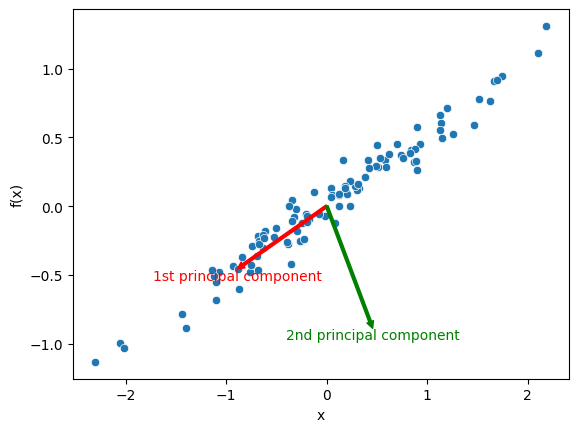
\includegraphics[width=7.2cm]{images/task1-1-1.png}
    \caption{The dataset with computed principle components on the image data}
    \label{fig:task1-1-1}
\end{figure}

The two principle components we obtained might not appear to be perpendicular to each other due to the aspect ratio of the image.

\bigskip
\noindent{\textbf{1.2 Image Data Compression}}

For the second part, we apply PCA to image data. We obtain the original gray-scale data with size (1024$\times$768) from the scipy.misc.face() method, and then rescale it into 249$\times$185, using interpolation from cv2.INTER\_CUBIC, provided in opencv-python package.

\begin{figure} [H]
    \centering
    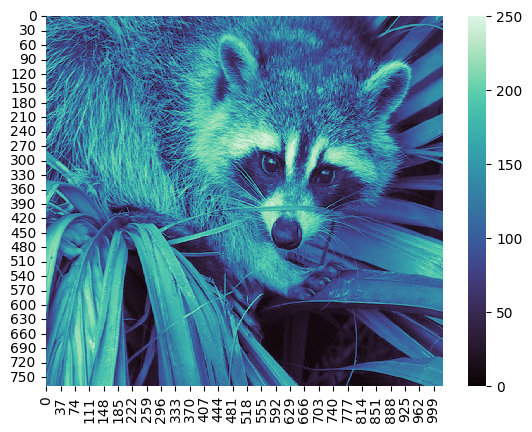
\includegraphics[width=6cm]{images/task1-2-1.png}
    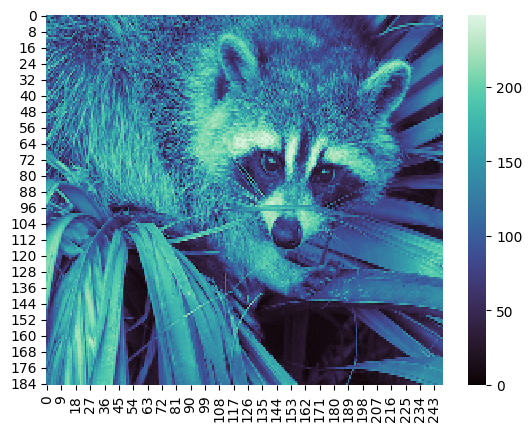
\includegraphics[width=6cm]{images/task1-2-2.png}
    \caption{The original (1024$\times$768) and rescaled (249$\times$185) image, represented in pseudo-color}
    \label{fig:task1-2-1}
\end{figure}

Using columns of the image as the
data points in PCA, we apply the same implemented algorithm, and calculate the energy, energy loss, and the number of principal components having energy loss through truncation smaller than the $1\%$ threshold, as is shown in figure \ref{fig:task1-2-loss}.

\begin{lstlisting}[language = Python, label={decoupling}]
U, S, VT = np.linalg.svd(data_bar)
size = S.size

energy = S*S/sum(S*S)
energy_loss = [] 
energy_loss_threshold = 0.01
energy_loss_index = size
for i in range(size):
    loss =  1-np.sum(energy[:i ])
    if loss < energy_loss_threshold and energy_loss_index == size:
        energy_loss_index = i
        flag = False
    energy_loss.append(loss)
\end{lstlisting}

\begin{figure} [H]
    \centering
    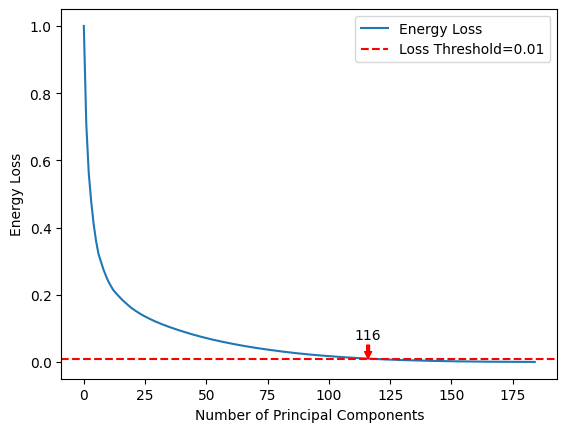
\includegraphics[width=9cm]{images/task1-2-loss.png}
    \caption{The energy loss with using different number of principal components}
    \label{fig:task1-2-loss}
\end{figure}

From which we can see that using more than 116 principle components can achieve to make the energy lost through truncation smaller than $1\%$. 

Now for the visualization, we apply the aforementioned PCA method to the rescaled image with all (185), 120, 50 and 10 principle components by truncating the $U, S, V^T$ matrices we got into corresponding sizes. The reconstructed images we got is shown in figure \ref{fig:task1-2-3}.

\begin{lstlisting}[language = Python, label={decoupling}]
U_r = U[:, :r]
S_r = S[:r]
VT_r = VT[:r, :]
\end{lstlisting}

\begin{figure} [H]
    \centering
    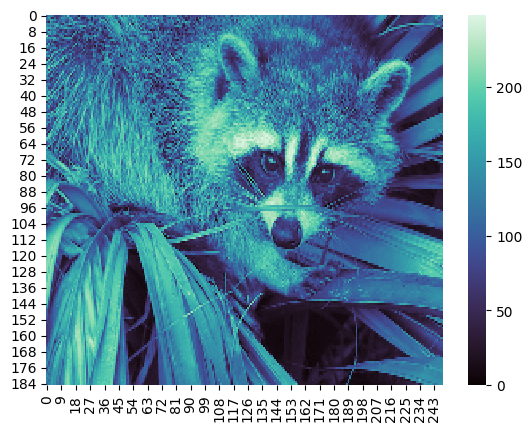
\includegraphics[width=7cm]{images/task1-2-185.png}
    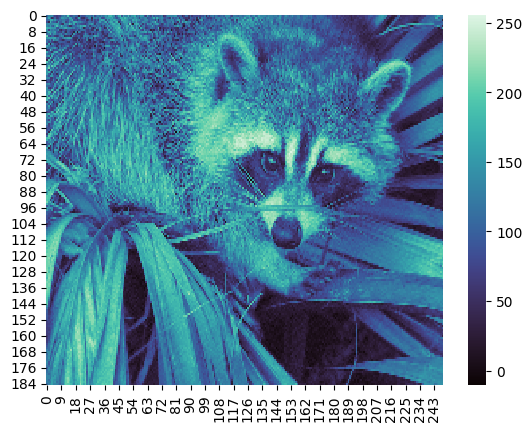
\includegraphics[width=7cm]{images/task1-2-120.png}
    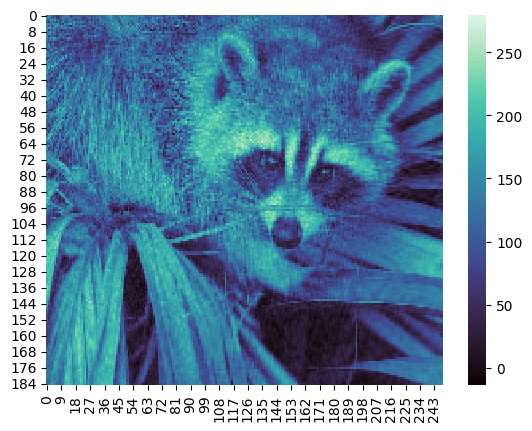
\includegraphics[width=7cm]{images/task1-2-50.png}
    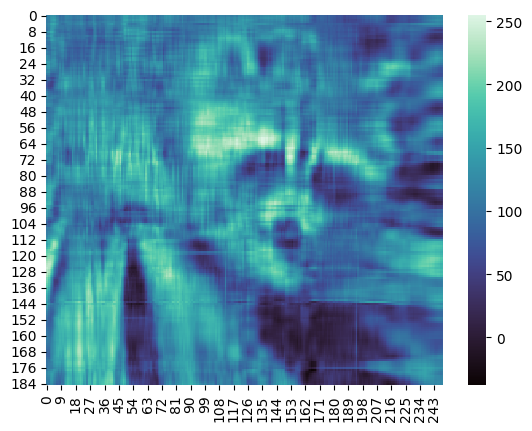
\includegraphics[width=7cm]{images/task1-2-10.png}
    \caption{The reconstructed images using 185 (upper left), 120 (upper right), 50 (lower left) and 10 (lower right) principle components}
    \label{fig:task1-2-3}
\end{figure}

As we can see the difference between the original image and reconstructed results using 185 (all) and 120 components is hardly visible, as their energy loss is all below the threshold of 0.01. Whereas many details of the image reconstructed from using 50 principle components are lost, such as the raccoon's hair, whiskers, and the edges of the surrounding foliage become blurred, while noticeable noise appears in large areas that should be smooth blocks of color. And the result using only 10 components is almost unrecognizable. 

\bigskip
\noindent{\textbf{1.3 Vadere Trajectory Data Compression}}

For this part, we are doing PCA on the trajectory data of 15 pedestrians over 1000 time steps. As the form the original data is provided, pedestrians' locations are stored on a 2-dimensional plane, therefore for each pedestrian, we consider their (x, y) coordinates as two independent variables within the time sequence. This can also be observed from visualizing the path of the first two pedestrians in the 2-dimensional space (figure \ref{fig:task1-3-1}).

\begin{figure} [H]
    \centering
    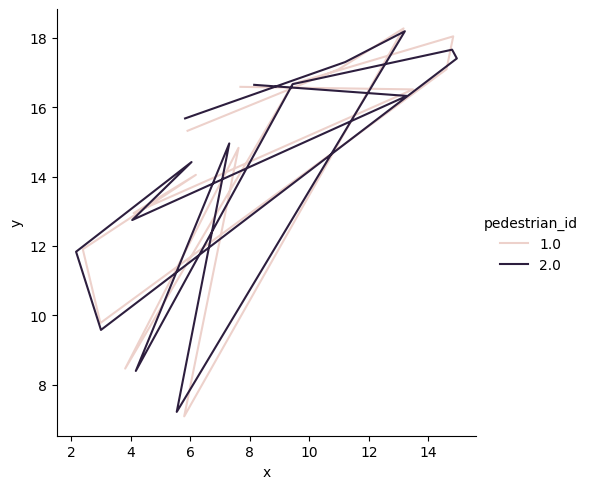
\includegraphics[width=7cm]{images/task1-3-1.png}
    \caption{The path of the first two pedestrians in the 2-dimensional space}
    \label{fig:task1-3-1}
\end{figure}

Hence we have a dataset with 30 variables and 1000 records. Now we apply PCA on this dataset and analyze the energy loss (figure \ref{fig:task1-3-loss}).

\begin{figure} [H]
    \centering
    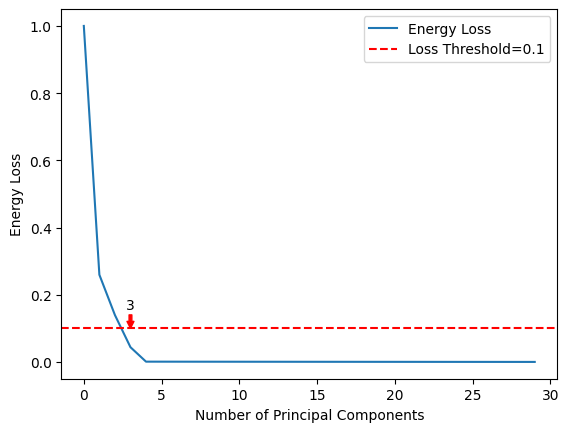
\includegraphics[width=9cm]{images/task1-3-loss.png}
    \caption{The energy loss with using different number of principle components on the trajectory data}
    \label{fig:task1-3-loss}
\end{figure}

\begin{figure} [H]
    \centering
    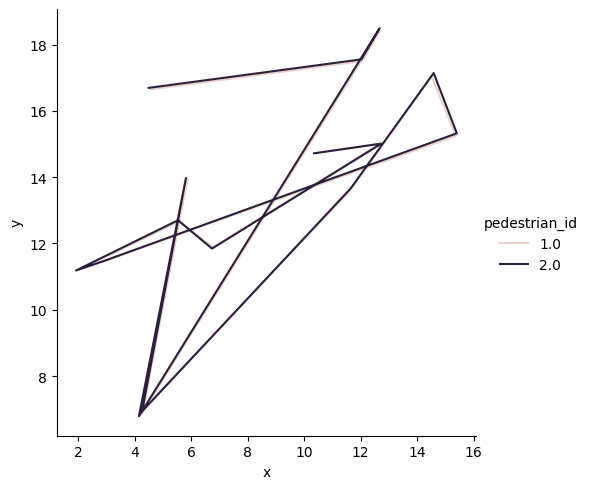
\includegraphics[width=5.2cm]{images/task1-3-2.png}
    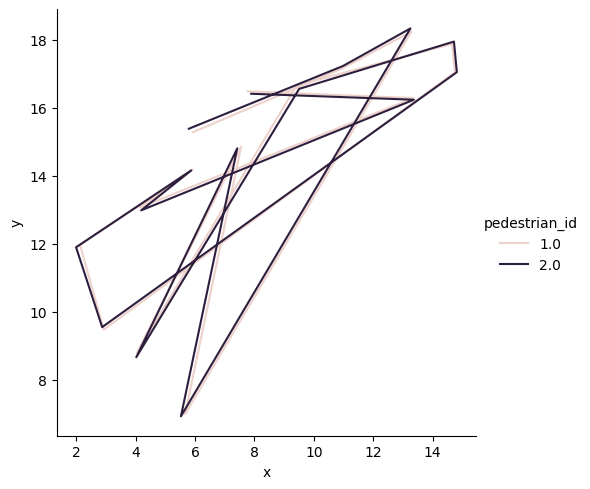
\includegraphics[width=5.2cm]{images/task1-3-3.png}
    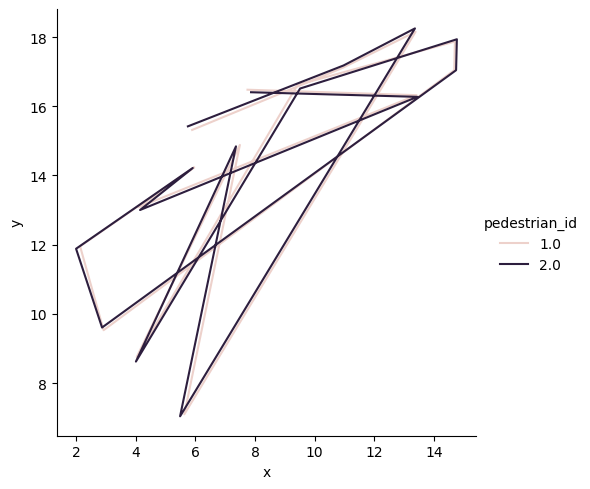
\includegraphics[width=5.2cm]{images/task1-3-4.png}
    \caption{The reconstructed path of the first two pedestrians in the 2-dimensional space using 2 (left), 3 (middle) and 4 (right) principal components}
    \label{fig:task1-3-2}
\end{figure}

From figure \ref{fig:task1-3-loss} we can see that two components are not enough to capture more than $90\%$ energy of the dataset. To do so, we need at least 3 principal components, which can reduce the loss lower below the threshold. 

The visualization result of the path of the first two pedestrians from both is shown in figure \ref{fig:task1-3-2}. The result with 2 principal components much deviates from the original curves, and the ones with 3 and 4 principal components are nearly identical to each other, both of which managed to capture a lot of details. Further increase the amount of principal components used can hardly improve the energy loss.
\bigskip
\end{task}

\newpage
\begin{task}{2: Diffusion Maps}

This algorithm was very clearly described in the statements, to implement it we just followed step by step the description. The implementation of the algorithm is located in the file DiffusionMaps.py and it takes as parameters the data and the number L + 1 of eigenfunctions wanted. As output, it returns two values: the eigenvector and the corresponding eigenvalues. For the distance matrix computation, we have followed the recommendation of using a sparse version and only considering points in a reasonable neighborhood, so we use the library scipy to implement the distance matrix.

It took us around two-three days to implement it and test it. To test it, we have used the library datafold to compare the results and plots. The plots obtained with our algorithm have the same shape of the ones obtained with the Diffusion Maps algorithm of the datafold library, although the values are slightly different. We think this is maybe caused because the datafold uses another method to implement it. 

Finally, different from PCA that only performs well for datasets close to a hyperplane (linear dimensionality reduction method), Diffusion Maps can reduct datasets that are non-linear. Given data in a high-dimensional space, the method focus on discovering the underlying manifold (lower-dimensional constrained "surface" upon which the data is embedded). 
\bigskip

\noindent{\textbf{2.1 Similarity of Diffusion Maps and Fourier analysis}}

First, we have created the periodic data set with N = 1000 points given by 
\[
X = \{ x_k \in \mathbb R^2 \}_{k=1}^{N}, x_k = (cos(t_k),sin(t_k)), t_k = (2{\pi}k)/(N + 1)
\]
A plot of this data set in 3D (the two parameters of \(x_k\) and \(t_k\)) can be observed in the Figure \ref{fig:task2-1-1}. 

\begin{figure} [H]
    \centering
    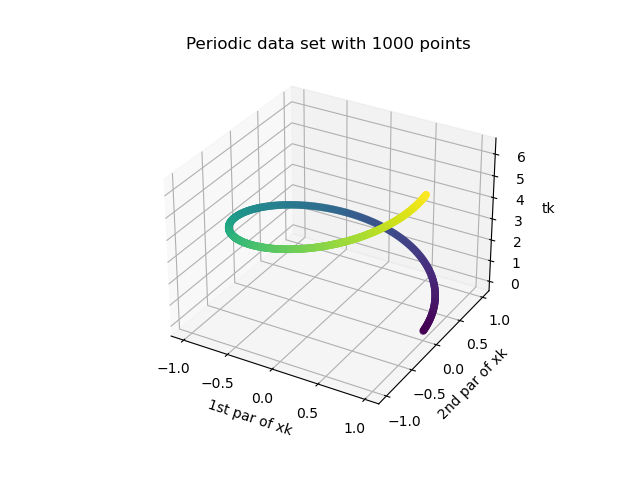
\includegraphics[width=10cm]{images/Dataset.png}
    \caption{Periodic data set of 1000 points}
    \label{fig:task2-1-1}
\end{figure}

After plotting the data set, the five eigenfuctions \(\phi_l \) associated to the largest eigenvalues \(\lambda_l \) have been computed with the Diffusion Maps algorithm on the periodic data set mentioned before. Below we can observe the five plots of the eigenfunctions \(\phi_l\)(\(x_k\)) (y-axis) against \(t_k\) (x-axis). 

\begin{figure} [H]
\centering
    \subfloat[]{
    \label{task2-1-2}
    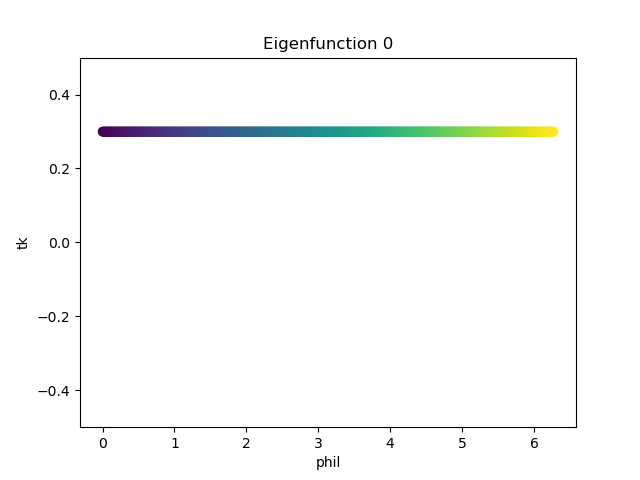
\includegraphics[width=0.33\textwidth]{images/plot0.png}}
    \subfloat[]{
    \label{task2-1-3}
    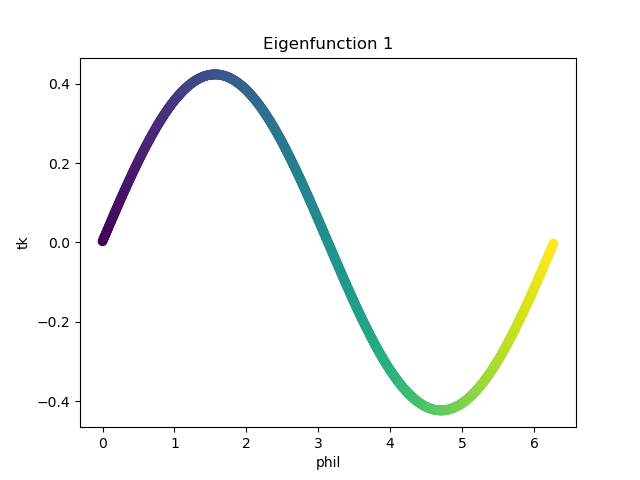
\includegraphics[width=0.33\textwidth]{images/plot1.png}}
    \subfloat[]{
    \label{task2-1-4}
    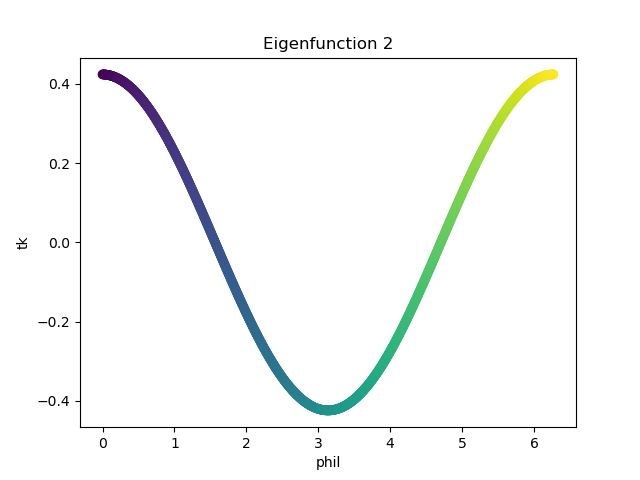
\includegraphics[width=0.33\textwidth]{images/plot2.png}}
    \label{s}
\end{figure}

\begin{figure} [H]
\centering
    \subfloat[]{
    \label{task2-1-5}
    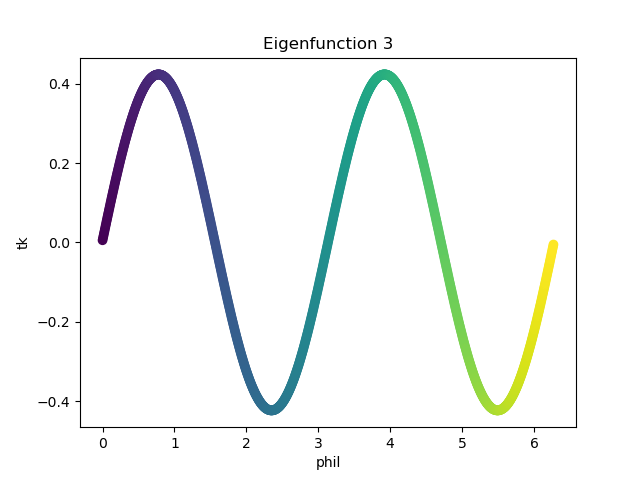
\includegraphics[width=0.33\textwidth]{images/plot3.png}}
    \subfloat[]{
    \label{task2-1-6}
    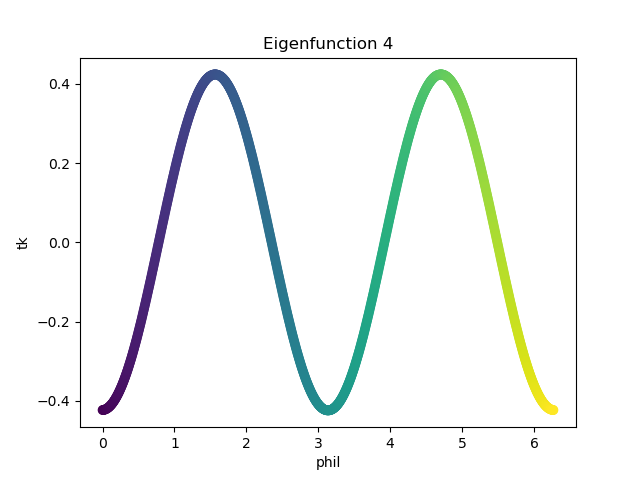
\includegraphics[width=0.33\textwidth]{images/plot4.png}}
    \caption{Plots of the values of the eigenfunctions against \(t_k\)}
    \label{d}
\end{figure}

Analysis: After observing the plots, we can see that the eigenfunction associated to the largest eigenvalue Figure \ref{task2-1-2} is constant while the others have a sinusoidal form, but with different period. And the Fourier transformations also converts periodic complex functions to combination of more simple sinusoidal functions. In conclusion, both methods tries to transform the original given data (that used to be complex periodic functions) to a combination of simple sinusoidal functions with different periods (or frequency).

\bigskip

\noindent{\textbf{2.2 Swiss roll manifold}}

First, with the sklearn Python library we have easily generated a Swiss roll data set with 5000 data points in three dimensional space. The Swiss roll manifold is defined through
\[
X = \{ x_k \in \mathbb R^3 \}_{k=1}^{N}, x_k = (u cos(u), v, u sin(u)),
\]

\noindent where (u, v) \(\in\) \([0, 10]^2\) are chosen uniformly at random. A plot of this data set can be observed in the Figure \ref{fig:task2-2-1}. 

\begin{figure} [H]
    \centering
    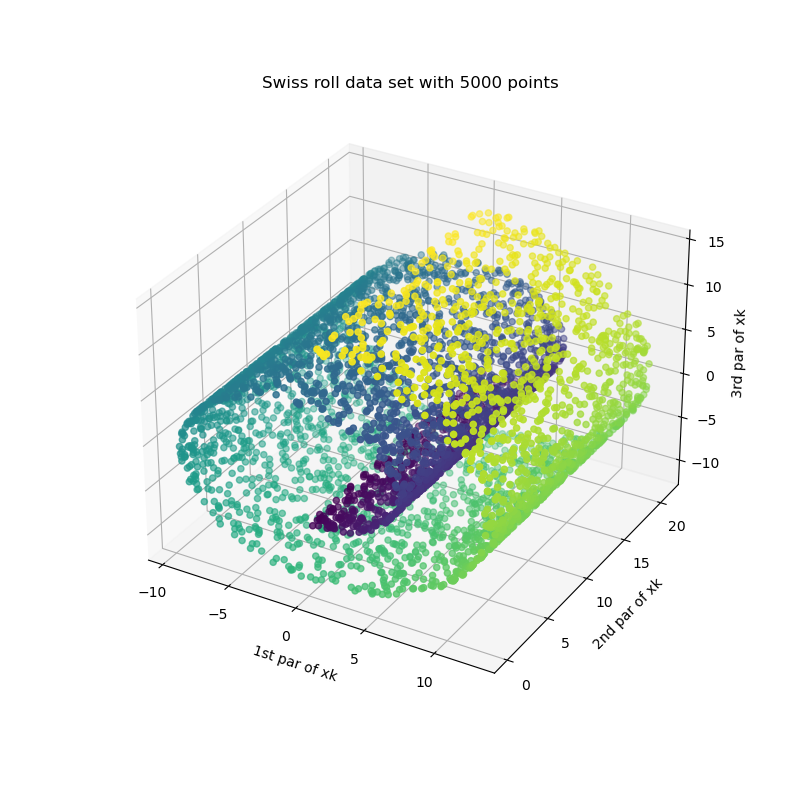
\includegraphics[width=10cm]{images/Swiss_roll_data_set.png}
    \caption{Swiss roll data set with 5000 points}
    \label{fig:task2-2-1}
\end{figure}

After that, we have obtained the first ten eigenfunctions of the Laplace Beltrami on the Swiss roll data set and observed that, in fact, the first non-constant eigenfunction was \(\phi_1 \), so next we have plotted the other eigenfunctions against this one in 2D plots (with \(\phi_1 \) in the horizontal axis). The plots can be observed in the next figure.

\newpage

\begin{figure} [H]
\centering
    \subfloat[]{
    \label{task2-2-2}
    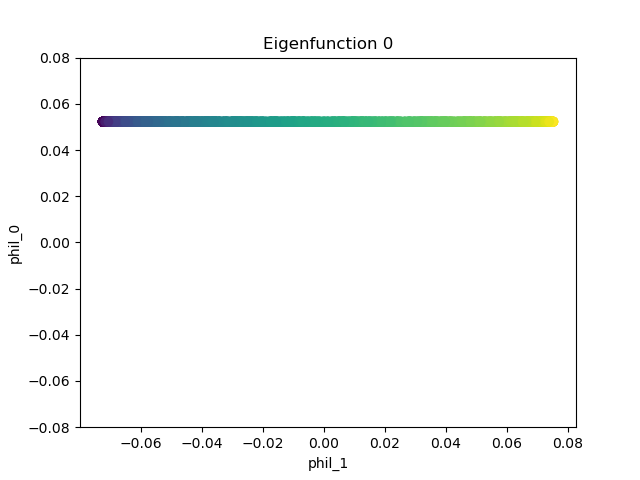
\includegraphics[width=0.33\textwidth]{images/Swiss_plot0.png}}
    \subfloat[]{
    \label{task2-2-3}
    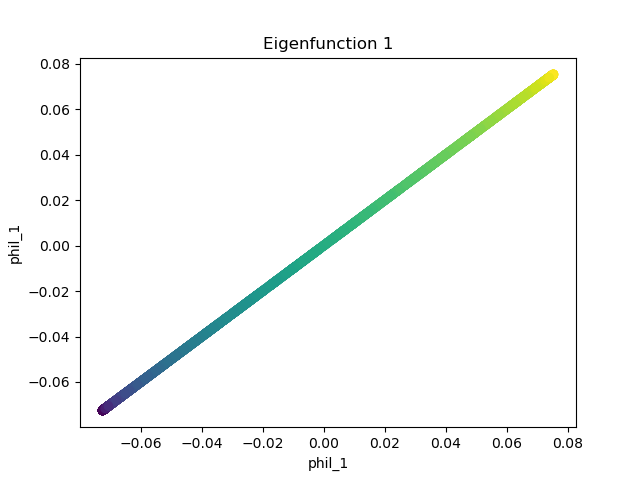
\includegraphics[width=0.33\textwidth]{images/Swiss_plot1.png}}
    \subfloat[]{
    \label{task2-2-4}
    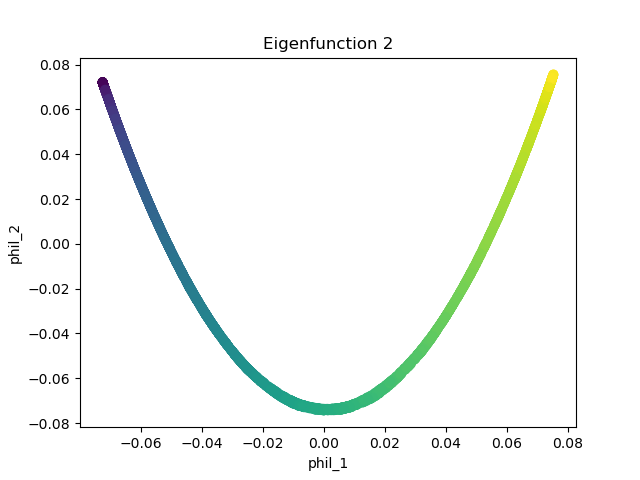
\includegraphics[width=0.33\textwidth]{images/Swiss_plot2.png}}
\end{figure}

\begin{figure} [H]
\centering
    \subfloat[]{
    \label{task2-2-5}
    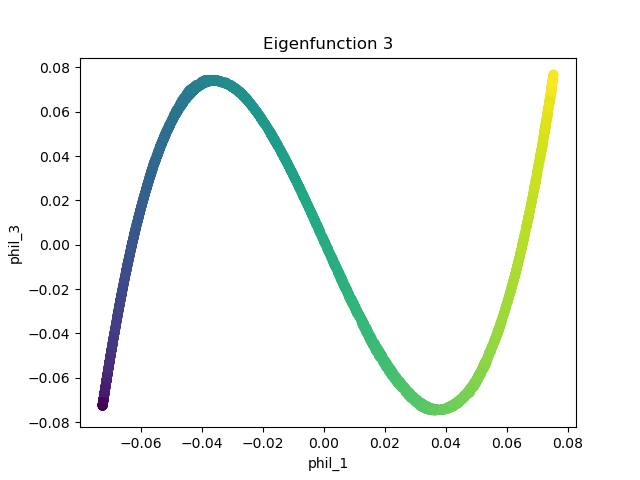
\includegraphics[width=0.33\textwidth]{images/Swiss_plot3.png}}
    \subfloat[]{
    \label{task2-2-6}
    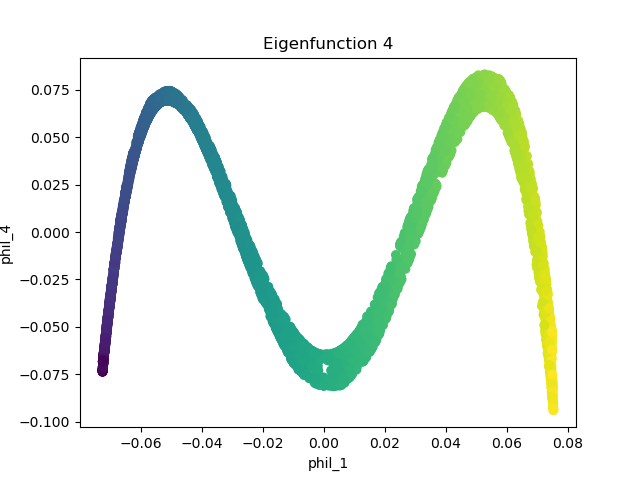
\includegraphics[width=0.33\textwidth]{images/Swiss_plot4.png}}
    \subfloat[]{
    \label{task2-2-7}
    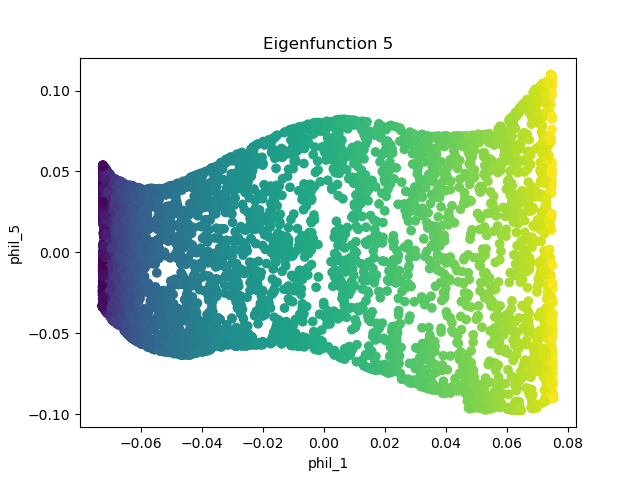
\includegraphics[width=0.33\textwidth]{images/Swiss_plot5.png}}
\end{figure}

\begin{figure} [H]
\centering
    \subfloat[]{
    \label{task2-2-8}
    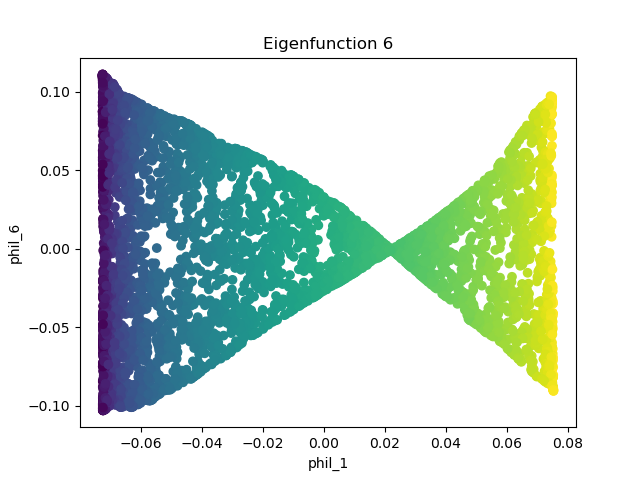
\includegraphics[width=0.33\textwidth]{images/Swiss_plot6.png}}
    \subfloat[]{
    \label{task2-2-9}
    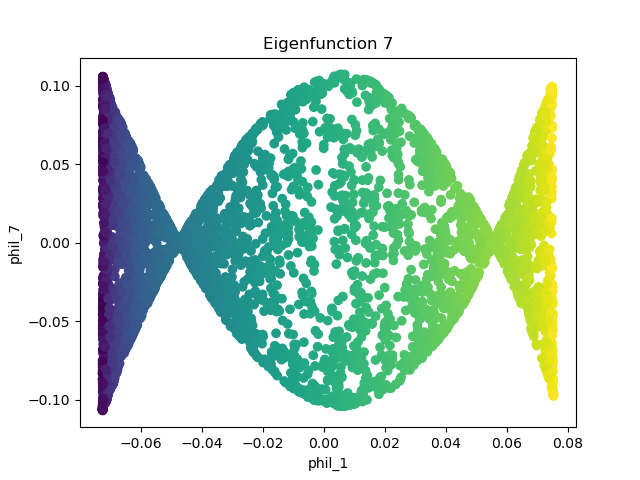
\includegraphics[width=0.33\textwidth]{images/Swiss_plot7.png}}
    \subfloat[]{
    \label{task2-2-10}
    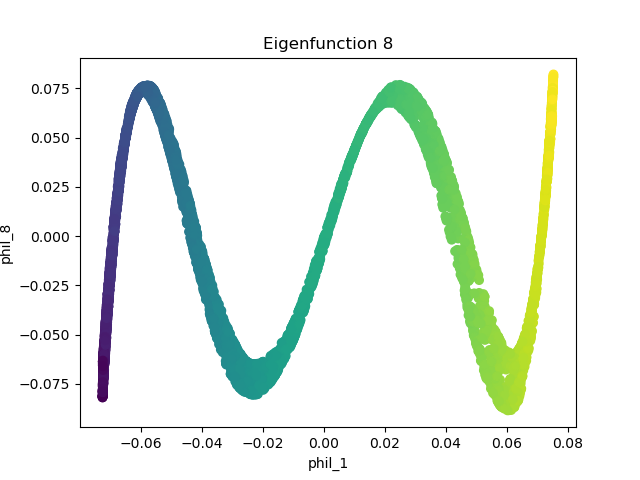
\includegraphics[width=0.33\textwidth]{images/Swiss_plot8.png}}
\end{figure}

\begin{figure} [H]
\centering
    \subfloat[]{
    \label{task2-2-11}
    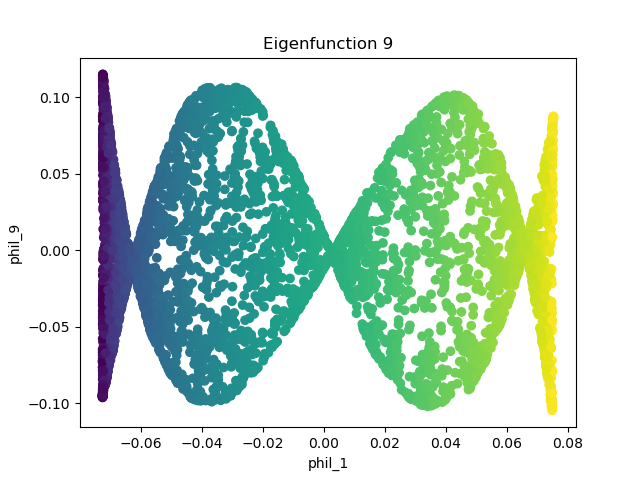
\includegraphics[width=0.33\textwidth]{images/Swiss_plot9.png}}
    \caption{Plots of the eigenfunction \(\phi_1\) against the others (5000 data points)}
    \label{plots}
\end{figure}

As we can observe in the different plots, the first one \(\phi_0\) is constant, so after plotting it against \(\phi_1\) we obtain a straight line. Obviously \(\phi_1\) against \(\phi_1\) is a diagonal. \(\phi_2\) and \(\phi_3\) are still functions of \(\phi_1\) because each value of the x-axis (\(\phi_1\)) corresponds to one value of the y-axis (\(\phi_2\) or \(\phi_3\)). We don't have this one-one correspondence since \(\phi_4\) and so on. This method is only by looking visually at the graphs, but there is also another mathematically based method, this one uses the by using the Local Regression Selection method of the datafold software and gives us the results. The results it gives is that the first value of l is 5. It confuses us a little bit, because of course \(phi_5\) is not longer a function of \(phi_1\), but \(phi_4\) also have not that one-one correspondence during all the graph. The shape of \(phi_4\) does look like \(phi_3\) and we believe more to the numerical method, so, 5 is the first value of l such that \(\phi_5\) is not longer a function of \(\phi_1\). 

Next, we need to compute the three principal components of the Swiss roll data set. First, we decomposed the centred data matrix into singular vectors U, V and values S with the svd method. To check if these values are correct, we have reconstructed the initial data set with these values, and after plotting it, they are quite similar, so we have assumed that it is correct. The three principal components are located in the \(V^T\) vector and have the following values:
\begin{itemize}
  \item Principal Component 1: [ 0.33333601 -0.72495673  0.60276434]
  \item Principal Component 2: [-0.38033221 -0.68839766 -0.6176213 ]
  \item Principal Component 3: [-0.86269028  0.02337527  0.50519212]
\end{itemize} 

Regarding at the question why is it impossible to only use two principal components to represent the data is that we will loss a lot of energy just by removing one component as we can see in the plot of the Figure \ref{fig:task2-2-12} (removing the third principal component, by setting the corresponding value of the S vector to 0). So we need all three principal components for the Swiss roll data set in order to not lose energy and be able to visualize well the data set.

\begin{figure} [H]
    \centering
    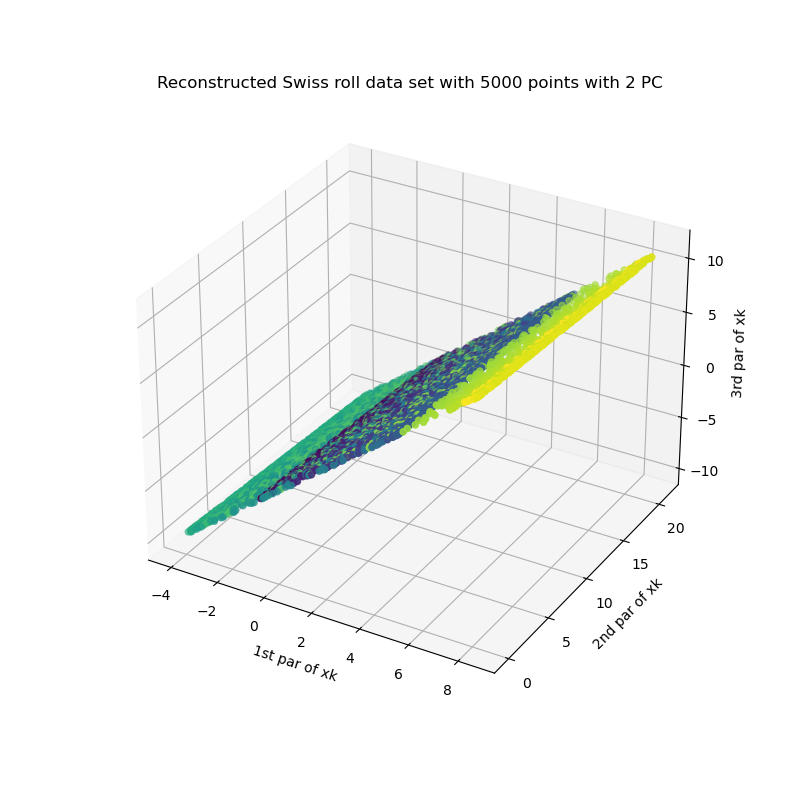
\includegraphics[width=10cm]{images/Swiss_plot_2_PC.png}
    \caption{Plot of the Swiss roll data set with 2 PC (5000 data points)}
    \label{fig:task2-2-12}
\end{figure}

The final question of this part is about what happens if only 1000 data points are used. 

\noindent First, let's analyse it for the Diffusion Maps. Visualizing the plot of the data set (Figure \ref{fig:task2-2-13}), we can observe that obviously there are less points than the previous one so it is less representative of the manifold. Also this reduction of data points can be observed in the eigenfunctions plots created with the Diffusion Maps algorithm, where there are much more noise than the previous one as we can see in the Figure \ref{fig:task2-2-13}.

\begin{figure} [H]
    \centering
    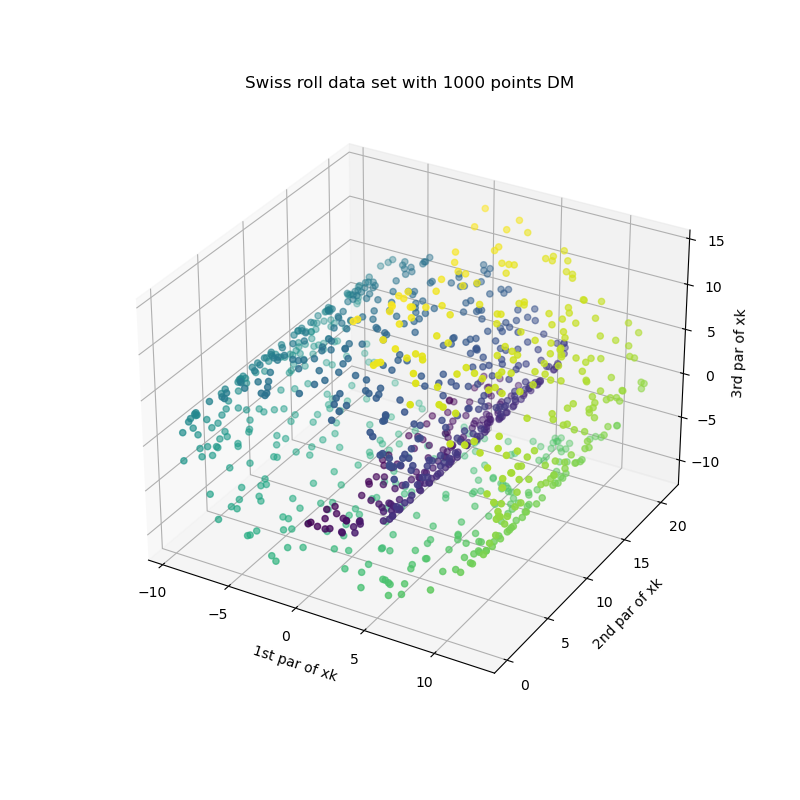
\includegraphics[width=10cm]{images/Swiss_roll_1000_data_set.png}
    \caption{Plot of the Swiss roll data set with DM (1000 data points)}
    \label{fig:task2-2-13}
\end{figure}

\newpage 

\begin{figure} [H]
\centering
    \subfloat[]{
    \label{task2-2-14}
    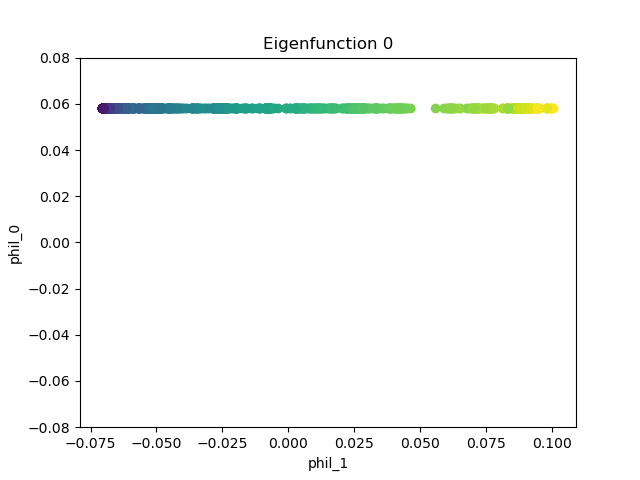
\includegraphics[width=0.33\textwidth]{images/Swiss_plot_10000.png}}
    \subfloat[]{
    \label{task2-2-15}
    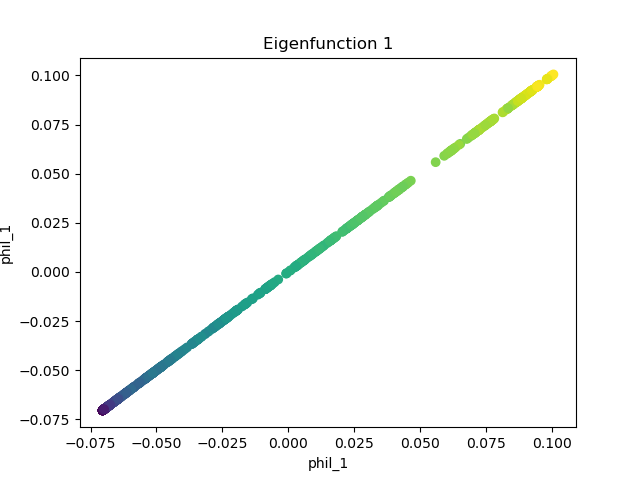
\includegraphics[width=0.33\textwidth]{images/Swiss_plot_10001.png}}
    \subfloat[]{
    \label{task2-2-16}
    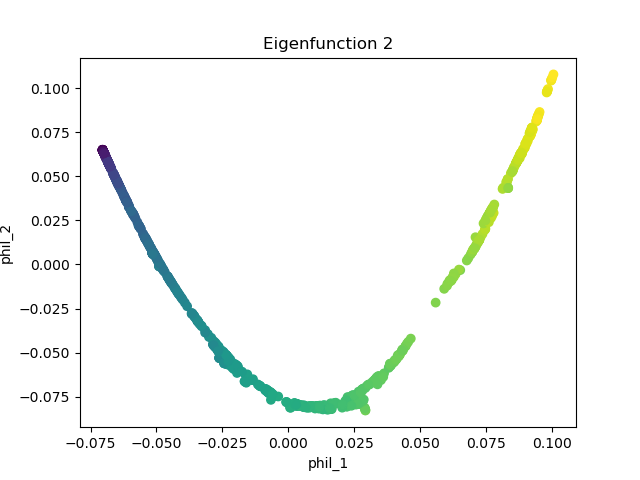
\includegraphics[width=0.33\textwidth]{images/Swiss_plot_10002.png}}
\end{figure}

\begin{figure} [H]
\centering
    \subfloat[]{
    \label{task2-2-17}
    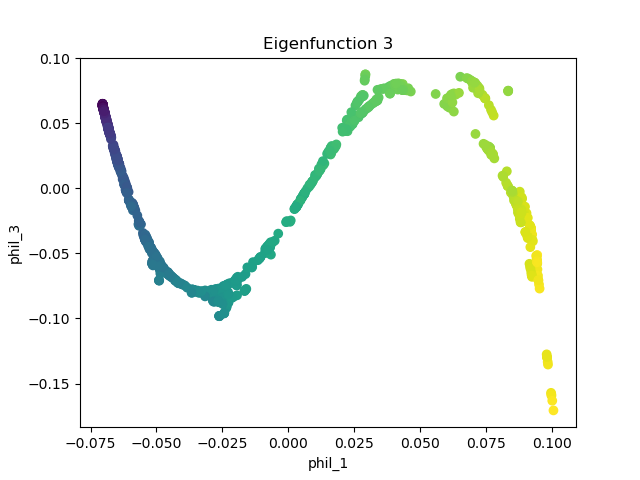
\includegraphics[width=0.33\textwidth]{images/Swiss_plot_10003.png}}
    \subfloat[]{
    \label{task2-2-18}
    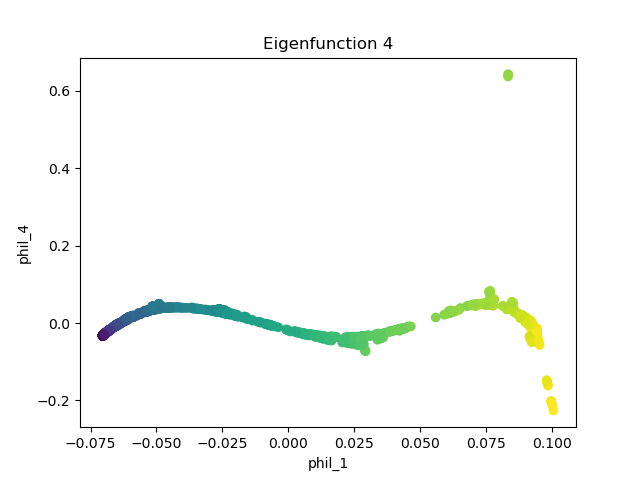
\includegraphics[width=0.33\textwidth]{images/Swiss_plot_10004.png}}
    \subfloat[]{
    \label{task2-2-19}
    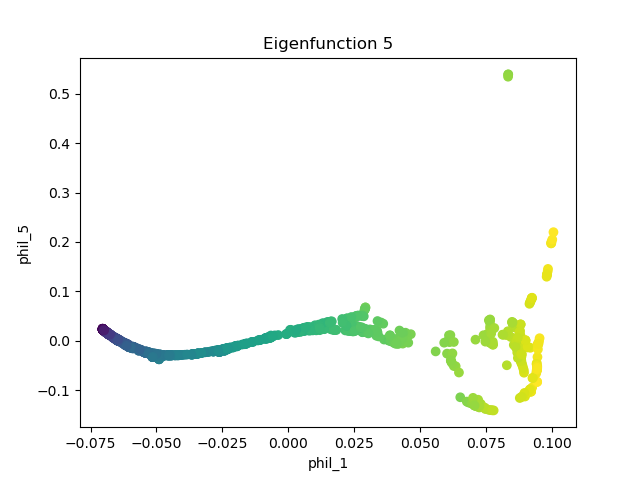
\includegraphics[width=0.33\textwidth]{images/Swiss_plot_10005.png}}
\end{figure}

\begin{figure} [H]
\centering
    \subfloat[]{
    \label{task2-2-20}
    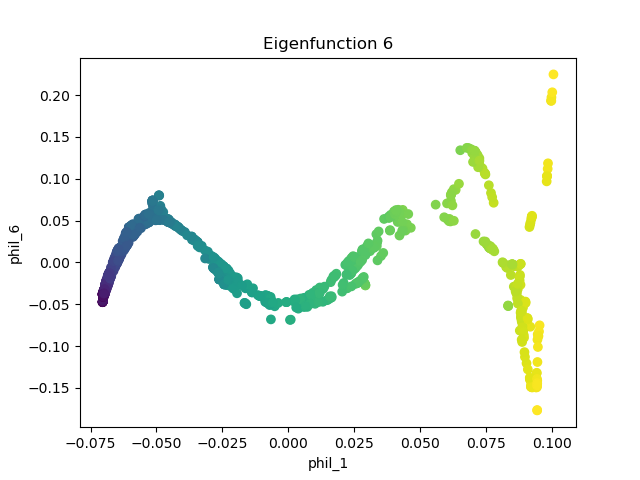
\includegraphics[width=0.33\textwidth]{images/Swiss_plot_10006.png}}
    \subfloat[]{
    \label{task2-2-21}
    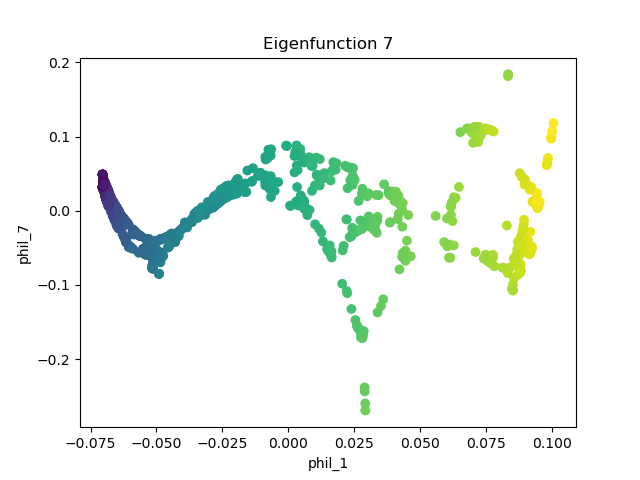
\includegraphics[width=0.33\textwidth]{images/Swiss_plot_10007.png}}
    \subfloat[]{
    \label{task2-2-22}
    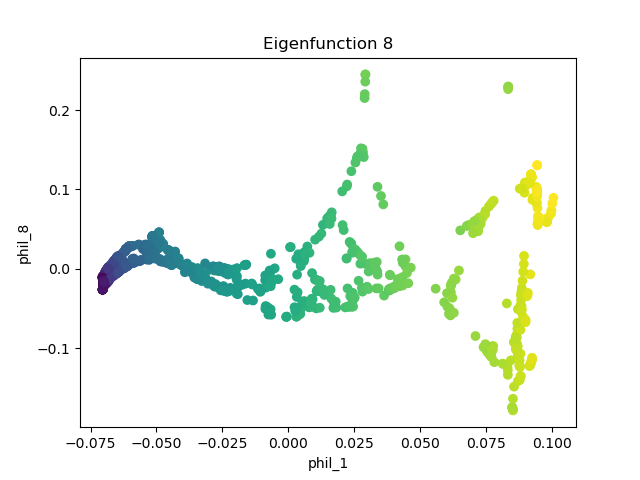
\includegraphics[width=0.33\textwidth]{images/Swiss_plot_10008.png}}
\end{figure}

\begin{figure} [H]
\centering
    \subfloat[]{
    \label{task2-2-23}
    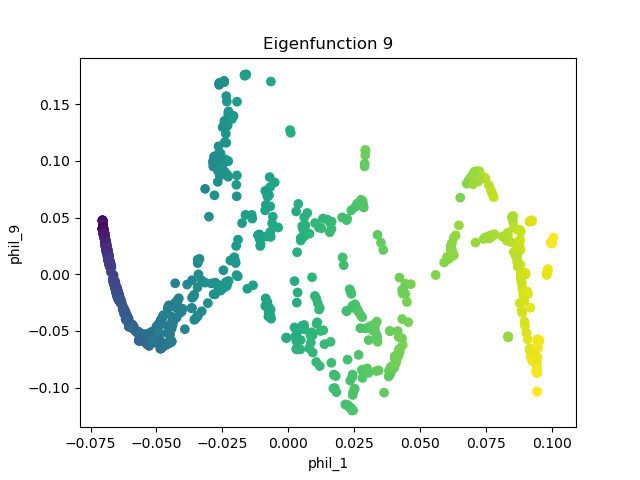
\includegraphics[width=0.33\textwidth]{images/Swiss_plot_10009.png}}
    \caption{Plots of the eigenfunction \(\phi_1\) against the others (1000 data points)}
    \label{plots}
\end{figure}

In the PCA case, again we have used the svd method to obtain the U and Vt vectors and the values S. By reconstructing it, the plot of the Figure \ref{fig:task2-2-13} has been obtained, so the same of the Diffusion Maps. As well as the previous case, it has three principal components, and it is not possible to just use two of them because again we will lose energy. A plot of the data set with 2 principal components can be observed in the next figure.

\begin{figure} [H]
    \centering
    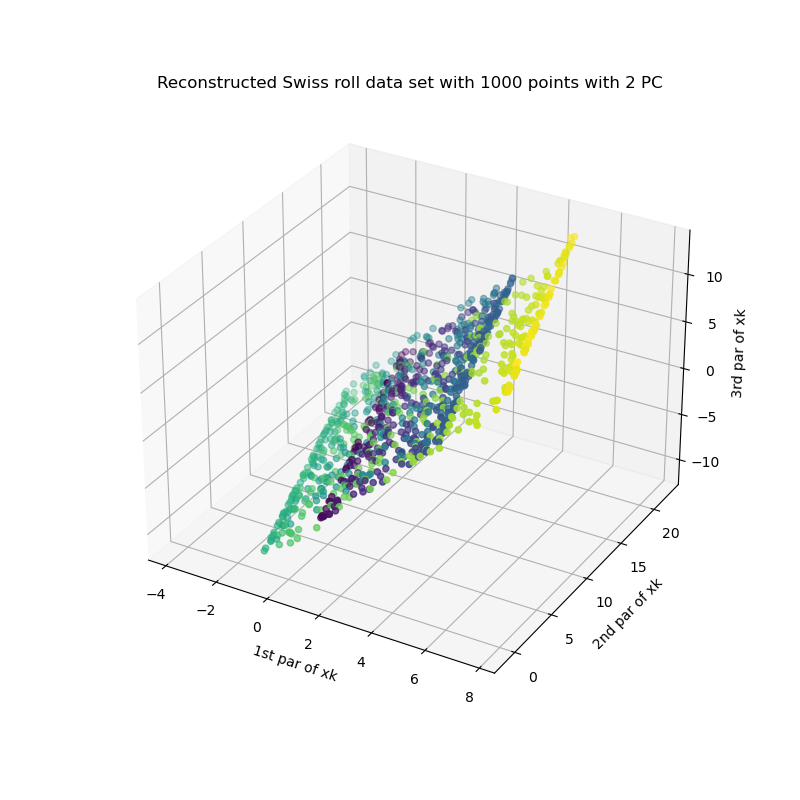
\includegraphics[width=10cm]{images/Swiss_plot_2_PC_1000.png}
    \caption{Plot of the Swiss roll data set with 2 PC (1000 data points)}
    \label{fig:task2-2-24}
\end{figure}

\bigskip

\noindent{\textbf{BONUS}}

The bonus consists on downloading the datafold software and compute the eigenvectors of the Swiss roll data set of the part 2, plot them against each other and analyze it. 

First, following the tutorial, we have generated the plot of the Swiss roll using 5000 data points, as we can see in the next figure:

\begin{figure} [H]
    \centering
    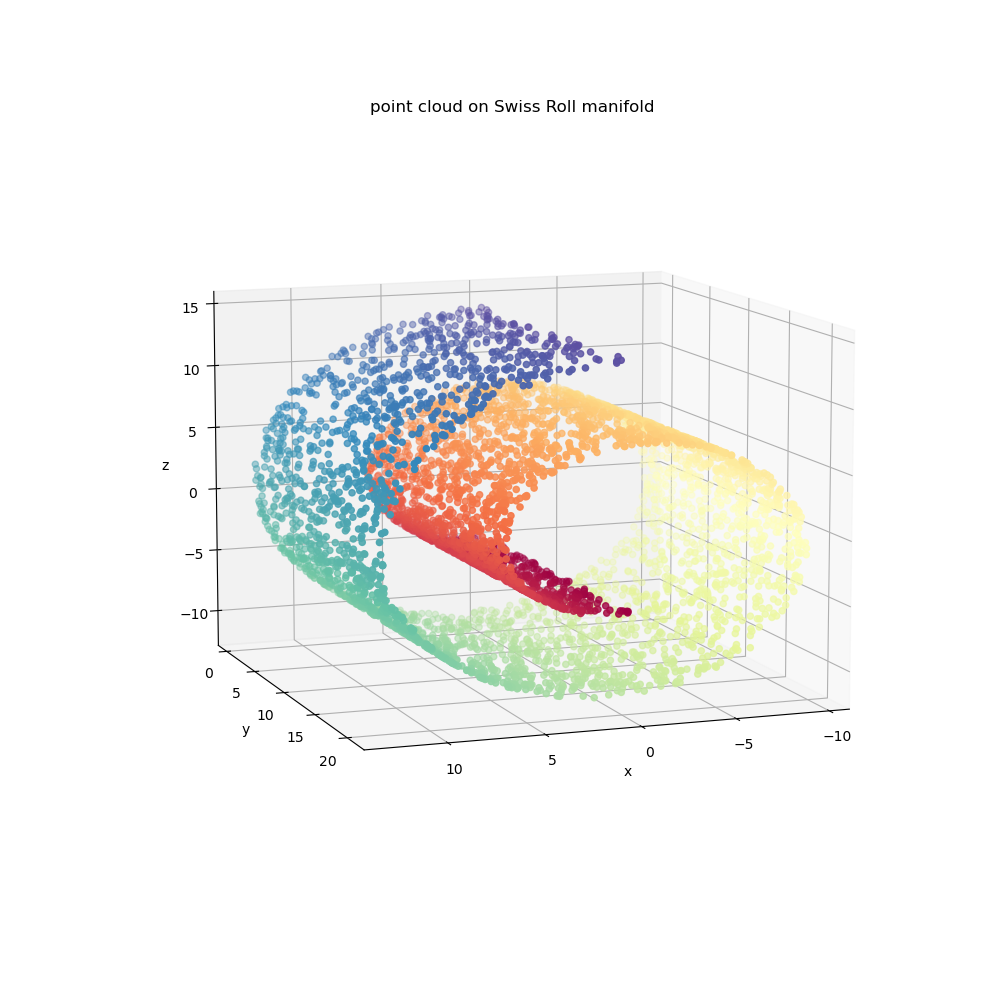
\includegraphics[width=10cm]{images/Swiss_plot_datafold.png}
    \caption{Plot of the Swiss roll data set generated with datafold (5000 data points)}
    \label{fig:bonus-1}
\end{figure}

The next step is to optimize the kernel parameters to get the epsilon and cut-off.

Next, we have fit a DiffusionMaps model of the datafold with the optimized parameters and then compared potential two-dimensions embeddings, as we have done in the part 2. The plots can be seen in the Figure \ref{fig:bonus-2}.

\begin{figure} [H]
    \centering
    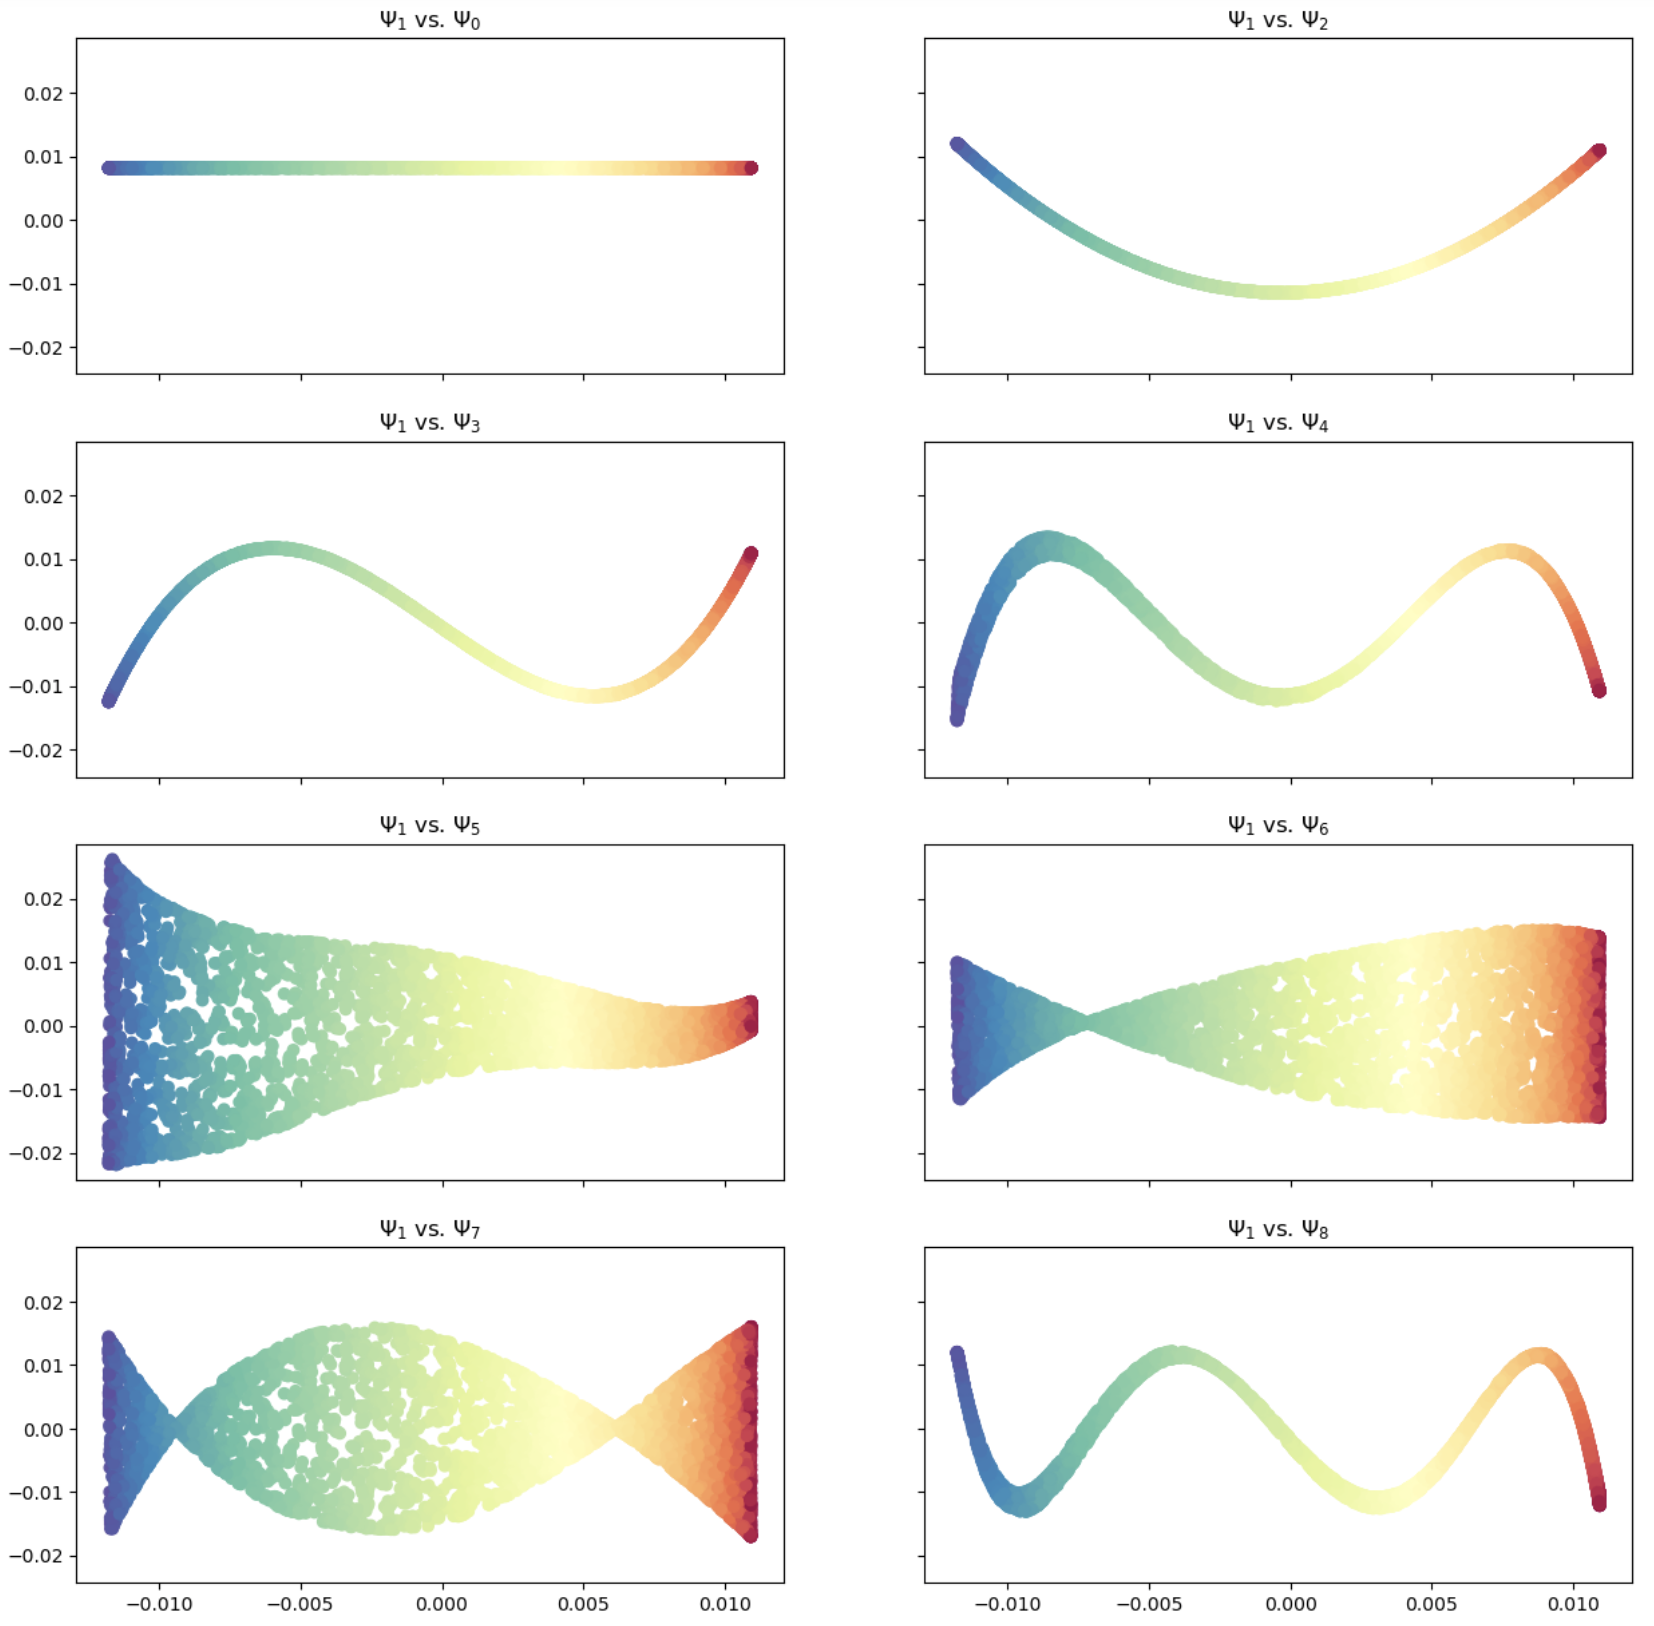
\includegraphics[width=10cm]{images/plots.png}
    \caption{Plots of the eigenfunction \(\phi_1\) against the others datafold version (5000 data points)}
    \label{fig:bonus-2}
\end{figure}

As can be observed, this plots are very similar to the ones we have obtained in the part 2. The same problem occurs here with the plot of the \(\phi_1\) against \(\phi_4\), where we can see an irregularity at the beginning of the plot, where there is no one-one corresponding. However, as before, using the Local Regression Selection, the first l such that \(\phi_l\) is not longer a function of \(\phi_1\) is again 5.

Finally, there is a plot of the unfolded point cloud:

\begin{figure} [H]
    \centering
    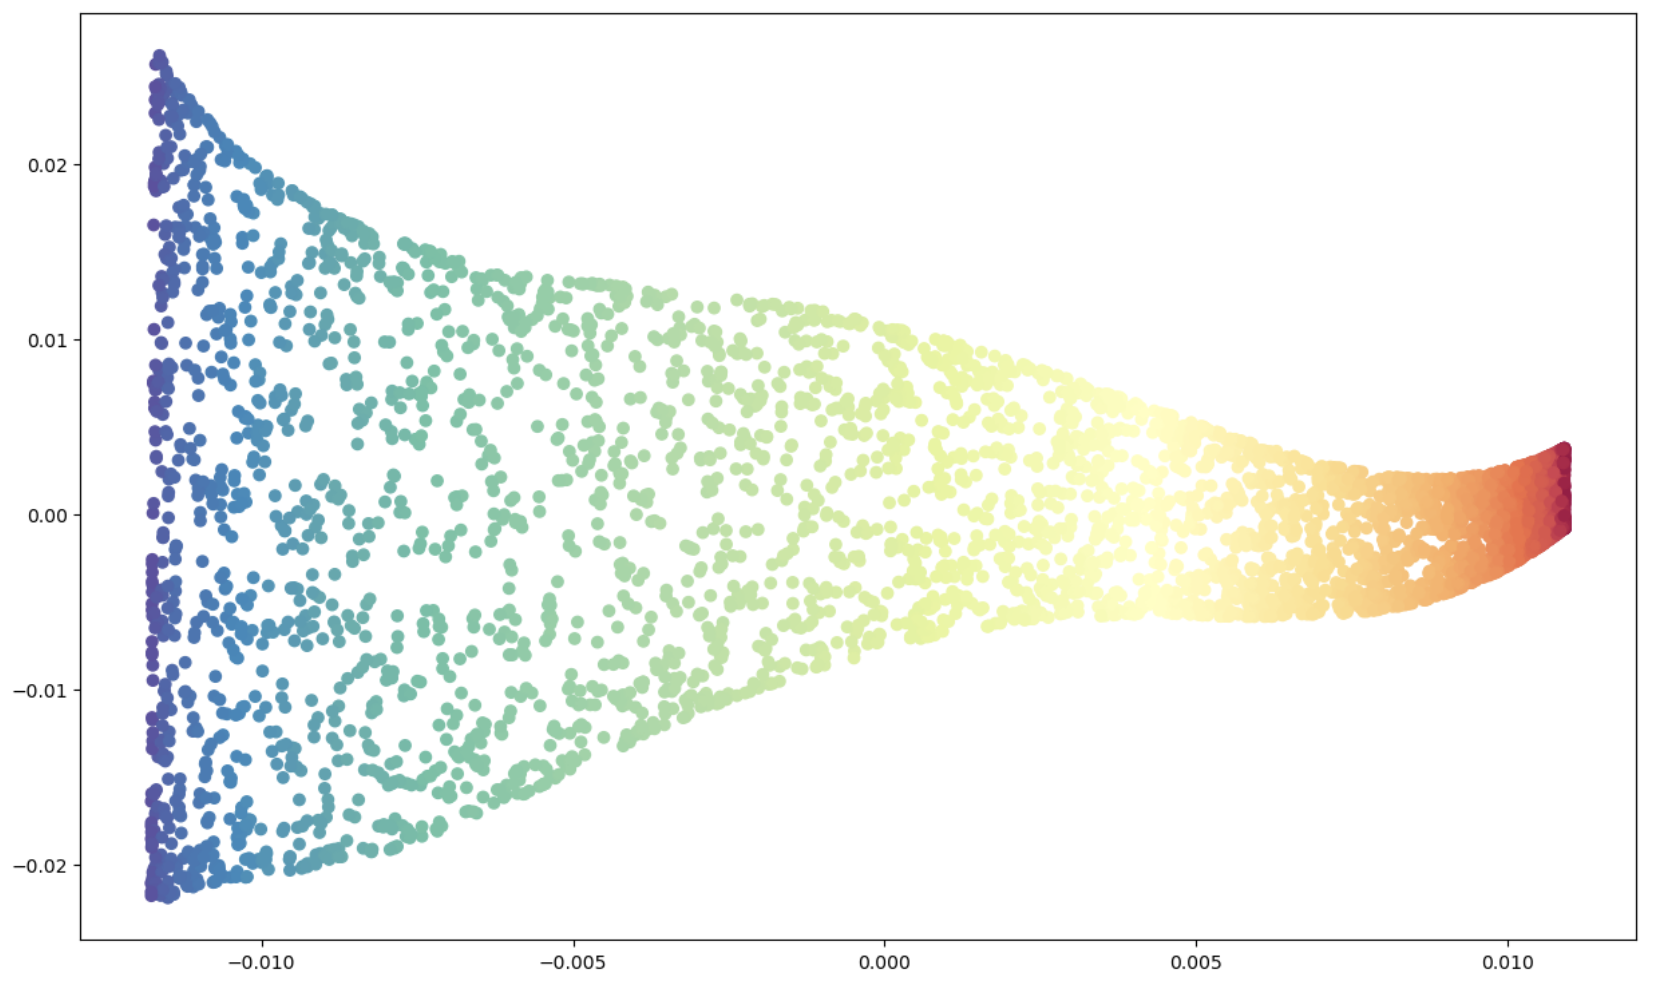
\includegraphics[width=10cm]{images/unfold.png}
    \caption{Unfolded point cloud of the Swiss roll data set}
    \label{fig:bonus-3}
\end{figure}

In conclusion, we have basically followed the steps of the tutorial and the results obtained are the expected ones, because they are almost the same than the ones we have obtained in the part 2 of the task.

\bigskip

\noindent{\textbf{2.3 Trajectory data analysis}}

In the last part of this task, we have to analyse the trajectory data in the file data\_DMAP\_PCA\_vadere.txt on Moodle as we did in the task 1, but in this case with Diffusion Map. Let's take a look at the path of the first two pedestrians in 2D space (Figure \ref{fig:task2-3-1})

\begin{figure} [H]
    \centering
    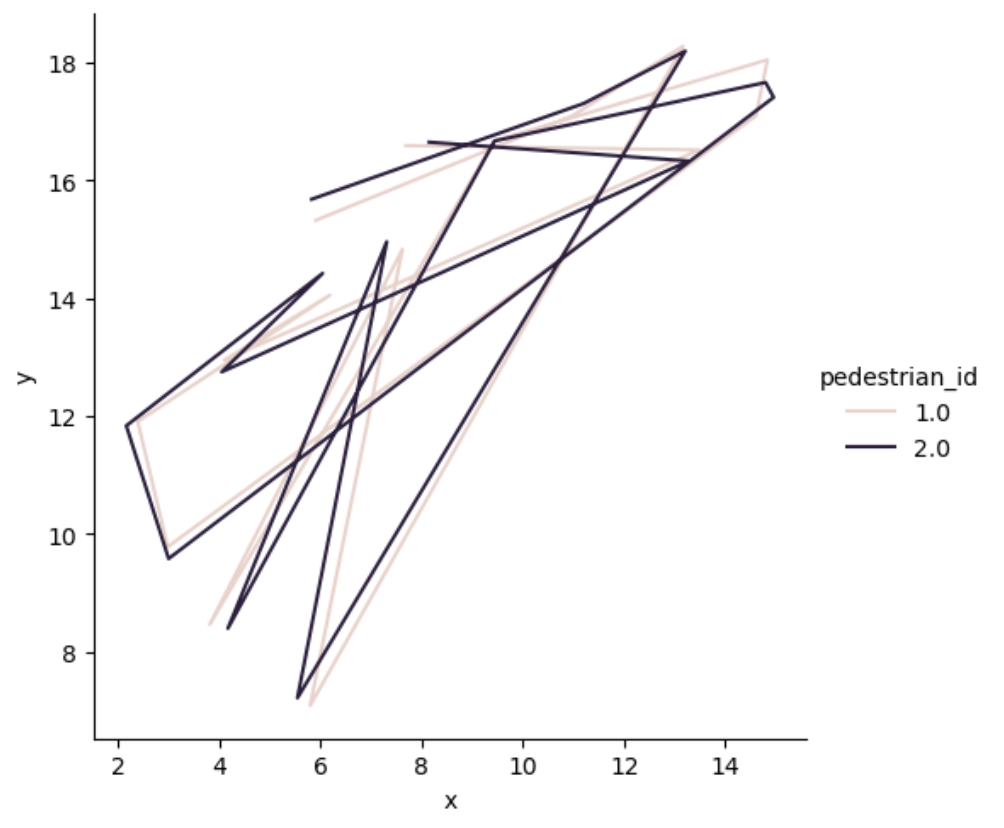
\includegraphics[width=10cm]{images/2d_plot.png}
    \caption{Path of the two pedestrians in 2D space}
    \label{fig:task2-3-1}
\end{figure}

We notice that Diffusion Maps do not have exactly the same energy interpretation of the eigenvalues (singular values) than PCA, so the task we have to do is finding a good combination of eigenfunctions to accurately represent the data set. A good combination of eigenfunctions is that one which leads to a subspace where there are no "intersections" of the curves of the unfold data.  

First, we have tried with 2 eigenfunctions in a range of 8 total eigenfunctions, the plots are shown below: 

\begin{figure} [H]
\centering
    \subfloat[]{
    \label{task2-3-2}
    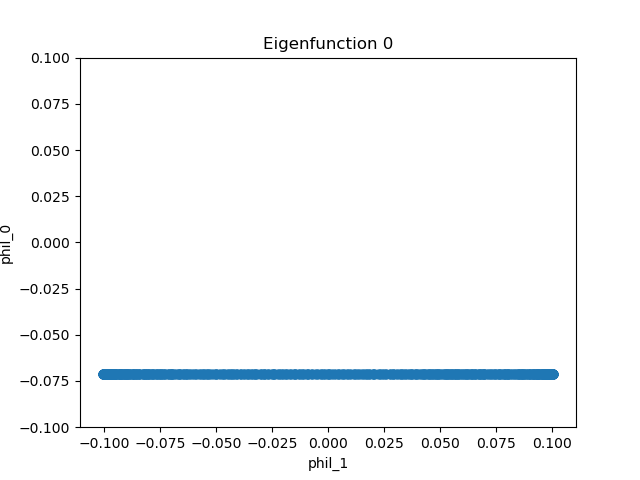
\includegraphics[width=0.33\textwidth]{images/plot_part_30.png}}
    \subfloat[]{
    \label{task2-3-3}
    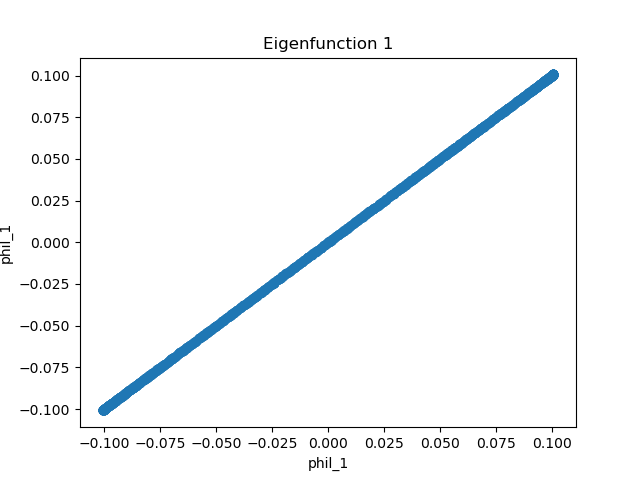
\includegraphics[width=0.33\textwidth]{images/plot_part_31.png}}
    \subfloat[]{
    \label{task2-3-4}
    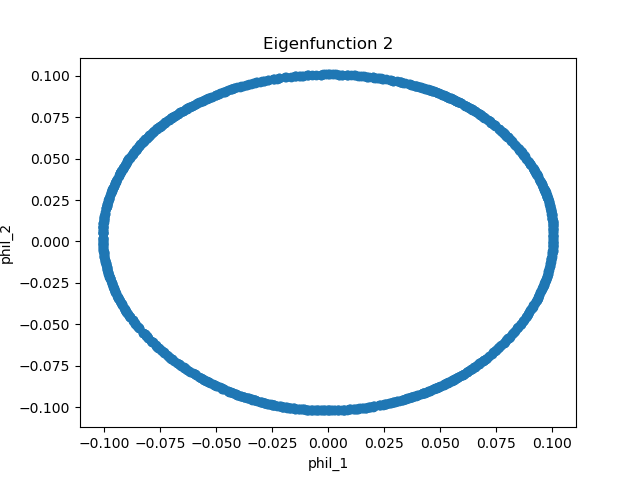
\includegraphics[width=0.33\textwidth]{images/plot_part_32.png}}
\end{figure}

\begin{figure} [H]
\centering
    \subfloat[]{
    \label{task2-3-5}
    \includegraphics[width=0.33\textwidth]{images/plot_part_33.png}}
    \subfloat[]{
    \label{task2-3-6}
    \includegraphics[width=0.33\textwidth]{images/plot_part_34.png}}
    \subfloat[]{
    \label{task2-3-7}
    \includegraphics[width=0.33\textwidth]{images/plot_part_35.png}}
\end{figure}

\begin{figure} [H]
\centering
    \subfloat[]{
    \label{task2-3-8}
    \includegraphics[width=0.33\textwidth]{images/plot_part_36.png}}
    \subfloat[]{
    \label{task2-3-9}
    \includegraphics[width=0.33\textwidth]{images/plot_part_37.png}}
    \caption{Plots of the eigenfunction \(\phi_1\) against the others}
    \label{plots}
\end{figure}

As we can observe in the plots, the eigenfunction \(\phi_1\) against the eigenfunction \(\phi_2\) is accurate to represent the data set because there are no "intersections" of the curves so just using two eigenfunctions it's enough to get a proper embedding. 

\bigskip
\end{task}



\newpage
\begin{task}{3: Training a Variational Autoencoder on MNIST}

\bigskip
This third task has been really challenging since it was our first time working with Variational Autoencoders while having little knowledge of statistics and deep learning. In fact, we could not implement the proper model of the VAE described in the exercise sheet. The implementation of the encoder was pretty clear. However, the decoder part and the ELBO loss was a bit tricky and we could not really understand it. In the end, after several days of trying to implementing it, we ended up following a tutorial which implementation was a bit different from what we were asked to do.

- What activation functions should be used for the mean and standard deviation of the approximate posterior and the likelihood—and why?

The standard deviation should be positive by convention, therefore positive-valued activation functions such as ReLU, Sigmoid, Softplus, etc. should be used for both the approximate posterior and the likelihood standard deviations. Moreover, for the standard deviation of the likelihood, since it is needed to calculate the density function and it is a divisor of this formula, a non-zero activation function must be used, such as Sigmoid.

As for the mean, since it can take any real value, it is not compulsory to use any activation function.

- What might be the reason if we obtain good reconstructed but bad generated digits?

The performance of the digit reconstruction and generation depends mainly on how well the latent space is modeled.

The reason for obtaining good reconstructed but bad generated digits might be due to a unbalance between the reconstruction and the KL divergence losses, more specifically for this case, the reconstruction being better than the KL divergence. This means that every input is well sampled in the latent space but badly distributed over the prior, which does not allow a good generation of digits from arbitrary points of this space, since it is very restricted to the training set used for modeling it.

\bigskip
\end{task}

\newpage
\begin{task}{4: Fire Evacuation Planning for the MI Building}

\bigskip
\end{task}

\newpage

\bibliographystyle{plain}
\bibliography{Literature}

\end{document}